\documentclass{article}
\usepackage[14pt]{extsizes}
\usepackage[utf8x]{inputenc}
\usepackage[russian]{babel}
\usepackage{enumitem}
\usepackage{paralist}
\usepackage{setspace}
\usepackage[left=3cm,right=2cm,top=2cm,bottom=2cm,bindingoffset=0cm]{geometry}
\usepackage{graphicx}
\graphicspath{{pictures/}}
\DeclareGraphicsExtensions{.pdf,.png,.jpg}
\setstretch{1,5}

\begin{document}
\textbf{\large Система верстки ТеХ (LaTeX).}

ТеХ — это система компьютерной вёрстки, предназначенная для набора научно-техническихтекстов высокого полиграфического качества.
Пользователь задает текст и его структуру с помощью определенных команд на языке низкоуровневой разметки, а ТеХ сам форматирует документ.

LaTeX — наиболее популярный набор макрорасширений ТеХа.
Главная идея LaTeX состоит в том, что авторы должны думать о содержании, не беспокоясь о конечном визуальном облике. Готовя свой документ, автор указывает логическую структуру текста (разбивая его на главы, разделы, таблицы, изображения), а LaTeX решает вопросы его отображения. 
Это и является основным отличем TeX от MS Word.
В первом случае используется парадигма WYSIWYM (What You See Is What You Mean), а во втором  — WYSIWYG (What You See Is What You Get).

~\

\textbf{Преимущества LaТеХ:}
\begin{compactitem}
\item Высокое качество подготовки научных текстов, работы с формулами;
\item Автоматическая рубрикация документа, нумерация формул, рисунков и списка литературы;
\item Пользователь сосредоточится на структуре, а не оформлении;
\item Внесение изменений в визуальное представление документа не требует изменения самого документа.
\end{compactitem}

~\

\textbf{Недостатки LaTeX:}
\begin{compactitem}
\item Для работы с данным средством требуется знать язык разметки;
\item Затуднена работа с рисунками;
\item В MS Word более простой и понятный интерфейс: что мы видим, то и получаем.
\end{compactitem}

\newpage

\textbf{\large Системы контроля версий.}

GitHub — крупнейший веб-сервис для хостинга IT-проектов и их совместной разработки. Основан на системе контроля версий Git.

Git — распределённая система управления версиями, обладающая всеми преимущствами РСКВ.

Существуют локальные, централизованные и распределенные системы контроля версий.
\textbf{Локальные СКВ} содержат простую базу данных, в которой хранятся все изменения нужных файлов. Эта утилита основана на работе с наборами патчей между парами версий. Но данный подход не позволялет сотрудничать с разработчиками за другими компьютерами, поэтому были созданы \textbf{централизованные СКВ}.

~\

\begin{figure}[h]
\center{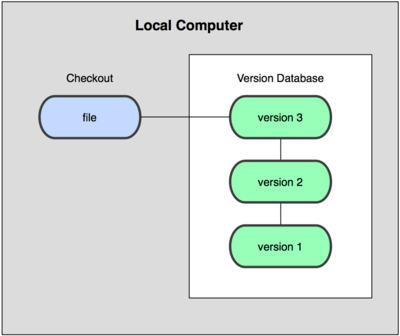
\includegraphics[scale=0.8]{1}}
\end{figure}

~\

Такие системы подразумевают центральный сервер, на котором хранятся все файлы. 
Центральный сервер — уязвимое место для всей системы. Есть риск потерять все данные, если поражается диск с центральной базой.

~\

\begin{figure}[h]
\center{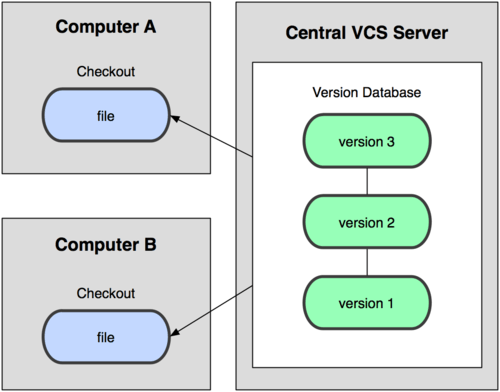
\includegraphics[scale=0.5]{2}}
\end{figure}

~\

Решением этой проблемы являются \textbf{распределенные СКВ}. В этих системах существуют удаленные и локальные репозитории.
Таким образом, клиенты не просто выгружают последние версии файлов, а копируют весь репозиторий, поэтому в случае отказа сервера база данных может быть восстановлена путем копирования клиентского репозитория.


\begin{figure}[h]
\center{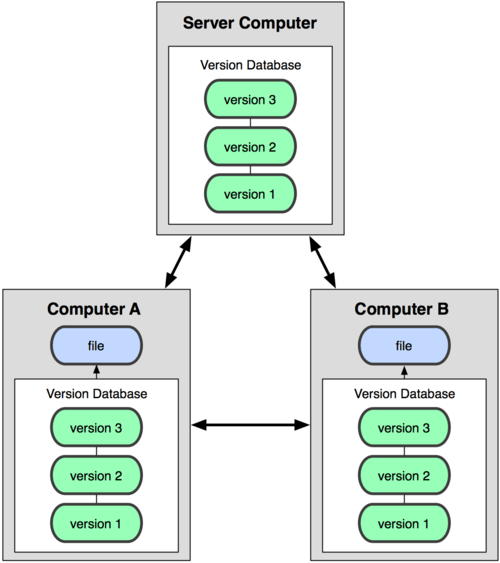
\includegraphics[scale=0.5]{3}}
\end{figure}

~\
Ядро Git представляет собой набор утилит командной строки с параметрами.
Репозиторий Git представляет собой каталог файловой системы, в котором находятся файлы конфигурации репозитория, файлы журналов, хранящие операции, выполняемые над репозиторием, индекс, описывающий расположение файлов и хранилище, содержащее собственно файлы. По умолчанию репозиторий хранится в подкаталоге с названием «.git» в корневом каталоге рабочей копии дерева файлов, хранящегося в репозитории. Любое файловое дерево в системе можно превратить в репозиторий git, отдав команду создания репозитория из корневого каталога этого дерева.

\newpage

\textbf{\large Транспортные протоколы UDP и TCP.}

Протоколы TCP и UDP относятся к транспортному уровню стека протоколов TCP/IP.
Основная функция этих протоколов – передача данных между прикладными
процессами, выполняющимися на узлах сети.

~\

\textbf{UDP}

Протокол UDP позволяет приложениям отправлять датаграммы без установления соединений. 
Полезен в ситуациях, когда не требуется обеспечение надежности доставки данных. 

~\

Заголовок UDP состоит из четырех полей по два байта:
\begin{compactitem}
\item  поле порта источника (source port);
\item поле порта пункта назначения (destination port);
\item поле длины (length);
\item поле контрольной суммы UDP (checksum UDP).
\end{compactitem}

~\

Протокол UDP ведет для каждого порта две очереди: очередь пакетов, поступающих в данный порт из сети, и очередь пакетов, отправляемых данным портом в сеть. 
Процедура обслуживания протоколом UDP запросов, поступающих от нескольких различных прикладных сервисов, называется мультиплексированием. 
Распределение протоколом UDP поступающих от сетевого уровня пакетов между набором высокоуровневых сервисов, идентифицированных номерами портов, называется демультиплексированием.

~\

Датаграммы, передаваемые с помощью UDP, могут быть утеряны, дублированы, прийти не по порядку. Но простота этого протокола обеспечивает его быстродействие и компактность.
Это широко применяется в клиент-серверных приложениях, когда клиент посылает запрос серверу и, если запрос или ответ теряется, пытается ещё раз через короткий промежуток времени.

~\

\textbf{ТСP}

Протокол TCP обеспечивает надежную транспортировку данных между прикладными процессами путем установления логического соединения.
 Благодаря логическому соединению TCP следит, чтобы передаваемые сегменты не были потеряны, не были продублированы и пришли к получателю в том порядке, в котором были отправлены.

~\

Заголовок TCP имеет размер 20 байт и содержит:
\begin{compactitem}
\item номер порта источника;
\item номер порта назначения;
\item последовательный номер - номер первого байта данных в сегменте;
\item номер подтверждения - следующий ожидаемый последовательный номер;
\item смещение данных - размер заголовка;
\item резерв - резервируются для будущего использования;
\item флаги - АСК (квитанция на принятый сегмент), URG, RST, SYN (первоначальное значение в поле номер последовательности) и т. д.
\item размер окна -содержит количество байт, которое может быть послано после байта, получение которого уже подтверждено;
\item контрольная сумма - по ней определяется, был ли искажен пакет;
\item указатель срочности;
\item опции - необязательные значения, которые указываются при необходимости;
\item заполнитель - здесь добавляется столько нулей, сколько необходимо, чтобы заголовок имел длину 32-бита.
\end{compactitem}

~\

В протоколе TCP правильность передачи каждого сегмента подверждается квитанцией от получателя.

~\

При установлении соединения обе стороны передают друг другу следующие параметры: максимальный размер сегмента, размер окна, начальный порядковый номер байта, с которого она начинает отсчет потока байтов. Для установлении соединения также используются флаги ACK, SYN, RST, FIN.

~\

Использованные источники:

- http://www.chin28.narod.ru/d10.1.htm 

- http://www.vanderboot.ru/tcp-ip/tcp-udp.php

- http://cdo.bseu.by/library/ibs1/net\_l/tcp\_ip/transp/tcp.htm

\end{document}